\documentclass[letterpaper,11pt]{article}
\usepackage[margin=1in]{geometry}
\usepackage[hyphens]{url}
\usepackage{colortbl}
\usepackage{listings}
\usepackage{graphicx}
\begin{document}

\date{\today}

\title{\Large \bf Memory Safety Bug Hunting with BAP} 

\author{Tiffany Bao, Dominic Chen, Rijnard van Tonder}

\maketitle

\section{Introduction}
\label{intro}

\paragraph{The Problem}

\paragraph{}
Although numerous debugging tools have been developed for performing static and
dynamic software analysis, the majority of these require access to source
code or utilization of special compile­time flags to embed debug information
within the output binary. In contrast, little effort has been spent on
developing static binary analysis tools which can directly analyze
off­the­shelf executables without executing them. For this project, we plan to
focus on a subset of common programming bugs that tend to introduce security
vulnerabilities, known as memory­safety errors. Examples of these include
buffer overflows, double frees, and uninitialized variables. In particular, we
define \emph{Security Outcomes} with respect to certain memory-safety errors,
and subsequently implement and test static analyses that yield these outcomes.
All analyses were written against our group's Binary Analysis Platform
(BAP) \cite{bap, brumley2011bap}.

\paragraph{}
A factor of this research area that appeals to many is the ability to
conclude whether vulnerabilities do or do not exist by performing
an analysis purely on the binary level. Due to the inherent difficulties
of operating at this level, %we can expand on what these difficulties are...
our approach to the problem starts out coarse, and continues to be
incrementally refined as we become more familiar with the numerous
barriers that inhibit vulnerability detection in binaries. In this respect,
we have much to say towards lessons learned in \S\ref{lessonslearned}.

\subsection{Approach Overview}
\label{approachoverview}

\paragraph{}
At the outset of this project, we planned to implement and test the static
analyses with respect to our original proposal:

\begin{enumerate}
  \item Intraprocedural data dependency resolution of instructions
  \item Intraprocedural detection of unchecked memory allocations
  \item Basic intraprocedural detection of buffer overflows in the stack
  \item Basic intraprocedural detection of buffer overflows in the heap
\end{enumerate}

\paragraph{}
Equipped with the knowledge of data flow dependency between instructions (1),
we determined to reason about various properties of typical vulnerabilities
that we could check (2-4). For example, we might like to follow how arguments
to a `strcpy` call are influenced by previous instructions as a function of
the stack register.

\subsection{Related Work}

\paragraph{}
Engler et. al. found numerous bugs with system-specific static analyses,
implemented by way of a meta-compilation language for the \texttt{gcc} compiler
\cite{dawson, dawson2}. Analyses are composed in the form of correctness rules
and automatic inference of rules form source code. Memory errors that are
checked include null pointer bugs, not checking allocation results, and uses of
freed pointers. This relates to our goal in that we would ideally like to perform
similar checks, albeit at the level of complexity of binary code. Whereas
Engler's work matured into a generic platform for specifying analyses, we must
start first with an ad-hoc approach to gain insight and familiarity in the
problem domain presented by binaries.

% needs more, TODO tiffany, dominic?

\subsection{Contributions}

Our key technical contributions are as follows:

\begin{enumerate}
  \item A dataflow analysis framework for BAP.
  \item General plugins for BAP that deliver
    \begin{enumerate}
      \item reaching definitions and
      \item data flow dependency resolution (use-def and def-use chains).
      \item registers corresponding to function call arguments and returns,
            according to the ARM ABI.
    \end{enumerate}
  \item Security-specific plugins for BAP that produce security outcomes by checking
    \begin{enumerate}
      \item whether memory allocation checks are performed on `memcpy`,
      \item whether calls such as strcpy are safe from buffer overflows under
        specific conditions, and
      \item whether malloc calls... % dominic?
    \end{enumerate}
  \item Results of testing the aforementioned plugins on the \texttt{GNU Coreutils}
    software suite.
\end{enumerate}

\subsection{Structure}

\paragraph{}
Due to the exploratory nature of this project on the binary level, we
concentrate much of our efforts on looking at viable approaches of analysis,
rather than optimizing properties of the analysis or testing against measurable
benchmarks. For this reason, it doesn't come as a surprise that our evaluation
section may be less expressive than our approach and ``lessons learned''.

\section{Approach}

\subsection{Overview}
\paragraph{}
Here we discuss our approach toward ensuring security properties as it evolved
over the course of the project. Initially, we determined to reason about each
of the cases in \S\ref{approachoverview} that relate to vulnerabilities
(2-4). To do so, we needed some basic infrastructure (1) which we describe
first. Thereafter, we describe our specific approaches to performing
security analyses with respect to specific \emph{Security Outcomes}.

\subsection{The Case for Reaching Definitions}

\paragraph{}
For example, consider the following code, where we desire to verify
that the return value of \texttt{malloc} is checked:

\begin{center}
\lstset{language=C, label=malloccheck,
caption=malloc.c, breaklines=true, basicstyle=\tiny, numbers=left}
\begin{lstlisting}
#include <stdlib.h>
#include <stdio.h>

int main() {
  // Uninitialized variable
  char *array = 0;


  array = malloc(32 * sizeof(*array));

  if (!array)
    return -1;

  free(array);

  return 0;
}
\end{lstlisting}
\end{center}

\paragraph{}
The disassembly of this binary might appear as follows (with two basic blocks,
before and after the call): 

\begin{center}
\lstset{language=C, label=mallocdisasm,
caption=Malloc disassembly, breaklines=true, basicstyle=\tiny, numbers=none}
\begin{lstlisting}
  begin(main_ENTRY) 
      000082c8: 04 e0 2d e5    str lr, [sp, #-4]! 
      000082cc: 20 00 a0 e3    mov r0, #0x20       
      000082d0: 49 00 00 eb    bl #0x124           ; call malloc
  end(main_ENTRY)
 
  begin(main_0xc) 
      000082d4: 00 00 50 e3    cmp r0, #0x0        ; check malloc return value
      000082d8: 02 00 00 0a    beq #0x8            
  end(main_0xc)
\end{lstlisting}
\end{center}

\paragraph{}
We would like to confirm that a check takes place after the call to malloc;
i.e., we would check for the presence of the \texttt{cmp} instruction and the
operand \texttt{r0} in \texttt{main\_0xc}.

\paragraph{}
However, it may easily be the case that the contents of \texttt{r0} are first
moved to another register, \texttt{r3}, which is subsequently checked by a
\texttt{cmp} instruction. In order to verify the buggy condition that the malloc
return value is never checked, we must verify that any flow of this data from
\texttt{r0} to other registers are also not checked. To obtain the statements
where \texttt{r0} data flows to, we make use of def-use chains. For the
definition of \texttt{r0} in the BIL IR, we check all uses of \texttt{r0} and
transitively look up the def-use chains for further registers, such as
\texttt{r3}, which the value in \texttt{r0} flows to. On the final set of
instructions, we verify that the data is subject to a \texttt{cmp} instruction.

\paragraph{}
This example demonstrates the need for def-use chains; our stack and heap based
analyses in turn also require use-def chains. Due to retreating edges in the
CFG, it is difficult to produce def-use chains given a single instruction. For
this reason we first implemented a dataflow framework and a
reaching-definitions pass. From the reaching definitions, we generate def-use
and use-def chains as necessary---e.g., we filter on those reaching definitions
which concern a particular use or def of a register.

\subsection{Data Flow Dependency}

\paragraph{}
An extension to the def-use and use-def chains was to produce the data (flow)
dependencies of a given statement in a forward or backward direction,
respectively. Essentially, given a register in a definition (such as a Move
instruction in the BIL IR), we can produce a set of all instructions that are
determined to transitively affect its value. We implement this
by way of a data dependency plugin for BAP. Consider the arguments to the
following \texttt{strcpy} call:

\begin{center}
\lstset{language=C, label=strcpy,
caption=strcpy.c, breaklines=true, basicstyle=\tiny, numbers=none}
\begin{lstlisting}
#include <stdio.h>
#include <string.h>

int main(int argc, char** argv) {
  char dst[10] = {0};
  strcpy(dst, argv[1]);
}
\end{lstlisting}
\end{center}

For the \texttt{dst} variable on the stack, encoded as an
\texttt{<address,statement>} pair, we have:

\begin{verbatim}
    <(0x8490:32, 0)> R0 := R2 
\end{verbatim}

The plugin will determine all preceding instructions it is dependent on:
\begin{verbatim}
    <(0x8444:32, 3)> SP := SP - 0x8:32
    <(0x8448:32, 2)> R11 := SP + 0x4:32
    <(0x848C:32, 2)> R2 := R11 - 0x10:32
\end{verbatim}

\paragraph{}
Now, we can observe the role that the stack pointer \texttt{SP} plays
when considering \texttt{dst}. A full listing of the BIL disassembly,
the data dependencies for \texttt{argv[1]}, and a graphical
output may be viewed in
the Appendix~\ref{appa}.

\subsection{Malloc Checking Security Outcomes}
% tiffany TODO

\subsection{Stack-based Security Outcomes}
\label{stackoutcomes}

\paragraph{}
A number of unfruitful approaches documented in~\S\ref{lessonslearned} lead us
to opting for an approach where we identify two properties which are important
from a security perspective, without inferring sizes of stack-based buffers.

\paragraph{\texttt{src} is a constant}
If we can determine that the \texttt{src} buffer is a constant, (and therefore
not dependent on any user input), the \texttt{strcpy} call is safe. While a
good property to check, it was found that a constant value corresponding to the
\texttt{src} argument didn't occur in practice. Depending on compiler
optimizations \texttt{strcpy} (as well as \texttt{sprintf} calls) would be
compiled to a \texttt{LDMIA.W} ARM instruction which directly copies memory.
Lastly, we observed that \texttt{strcpy} and \texttt{sprintf} may be replaced
by the \texttt{\_\_strcpy\_chk} and \texttt{\_\_sprintf\_chk} counterparts,
which are less interesting to analyse from a security standpoint.

\paragraph{}
Nevertheless, we implemented a partial check of this case in the plugin, and
assumed the standpoint that any \texttt{src} address originating from the
\texttt{ro.data} section implies a constant, fixed value. However, for this
check we only consider the statement which loads a value immediately before the
call, and not originating previous statements. % because memory and interfering statements

\paragraph{Stack accesses within the frame} 
For this outcome, we confirm that all instructions which access elements on
the stack, plus a fixed offset, are within the stack range of a function. We
infer the size of the frame by considering the statements that manipulate
SP in the function prologue. While we didn't observe any cases where the
stack range was exceeded, this type of check forms the basis for further,
more sophisticated improvements.

\subsection{Malloc-based Security Outcomes}
% dominic TODO




% ===============================================
\section{Experimental Setup}

\paragraph{}
Our experimental setup consisted of running our plugins with BAP \texttt{0.9.6}
\cite{bap} on a set of binaries, including GNU \texttt{Coreutils} and our
own examples.

\subsection{Unchecked Malloc}
% tiffany TODO

\subsection{Stack Check Plugin}

\paragraph{}
The stack check plugin was tested against the GNU \texttt{Coreutils} suite. We
primarily chose the \texttt{Coreutils} suite since a) it can be compiled for
ARM, and b) it contains numerous calls to \texttt{strcpy}, \texttt{memcpy},
\texttt{malloc}, and so forth.  The stack check plugin, while configurable,
concretely checked for function calls to:

\begin{itemize}
  \item \texttt{strcat}
  \item \texttt{strcpy}
  \item \texttt{strncpy}
  \item \texttt{memcpy}
\end{itemize}

\paragraph{}
The plugin collected a number of statistics on the binaries, including
the number of argument sites (that is, statements that set up registers
before a call), the number of functions which contained calls to `dangerous'
functions, and the maximum number of statements on which an argument
site statement was dependent. These are illustreated in Figure~\ref{fig:corestats}.

\begin{figure}[ht!]
\centering
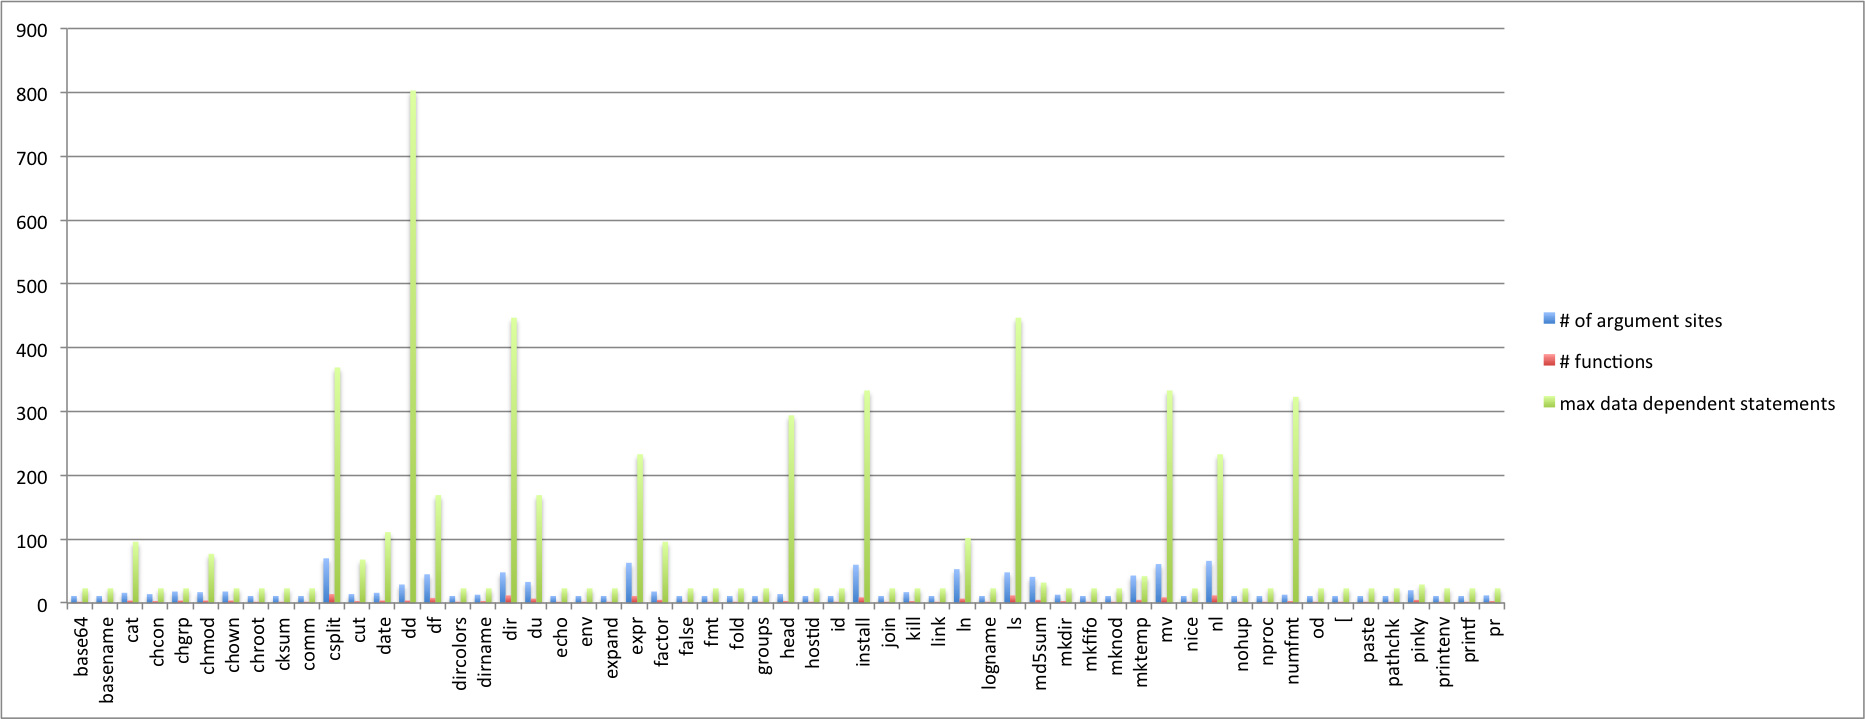
\includegraphics[scale=0.55, trim=0mm 0mm 0mm 0mm, clip]{img/coreutils2.pdf}
\caption{Coreutils statistics generated by plugin}
\label{fig:corestats}
\end{figure}

Figure~\ref{fig:coretotal} presents the total number of statements in a binary
which affect unique argument sites.

\begin{figure}[ht!]
\centering
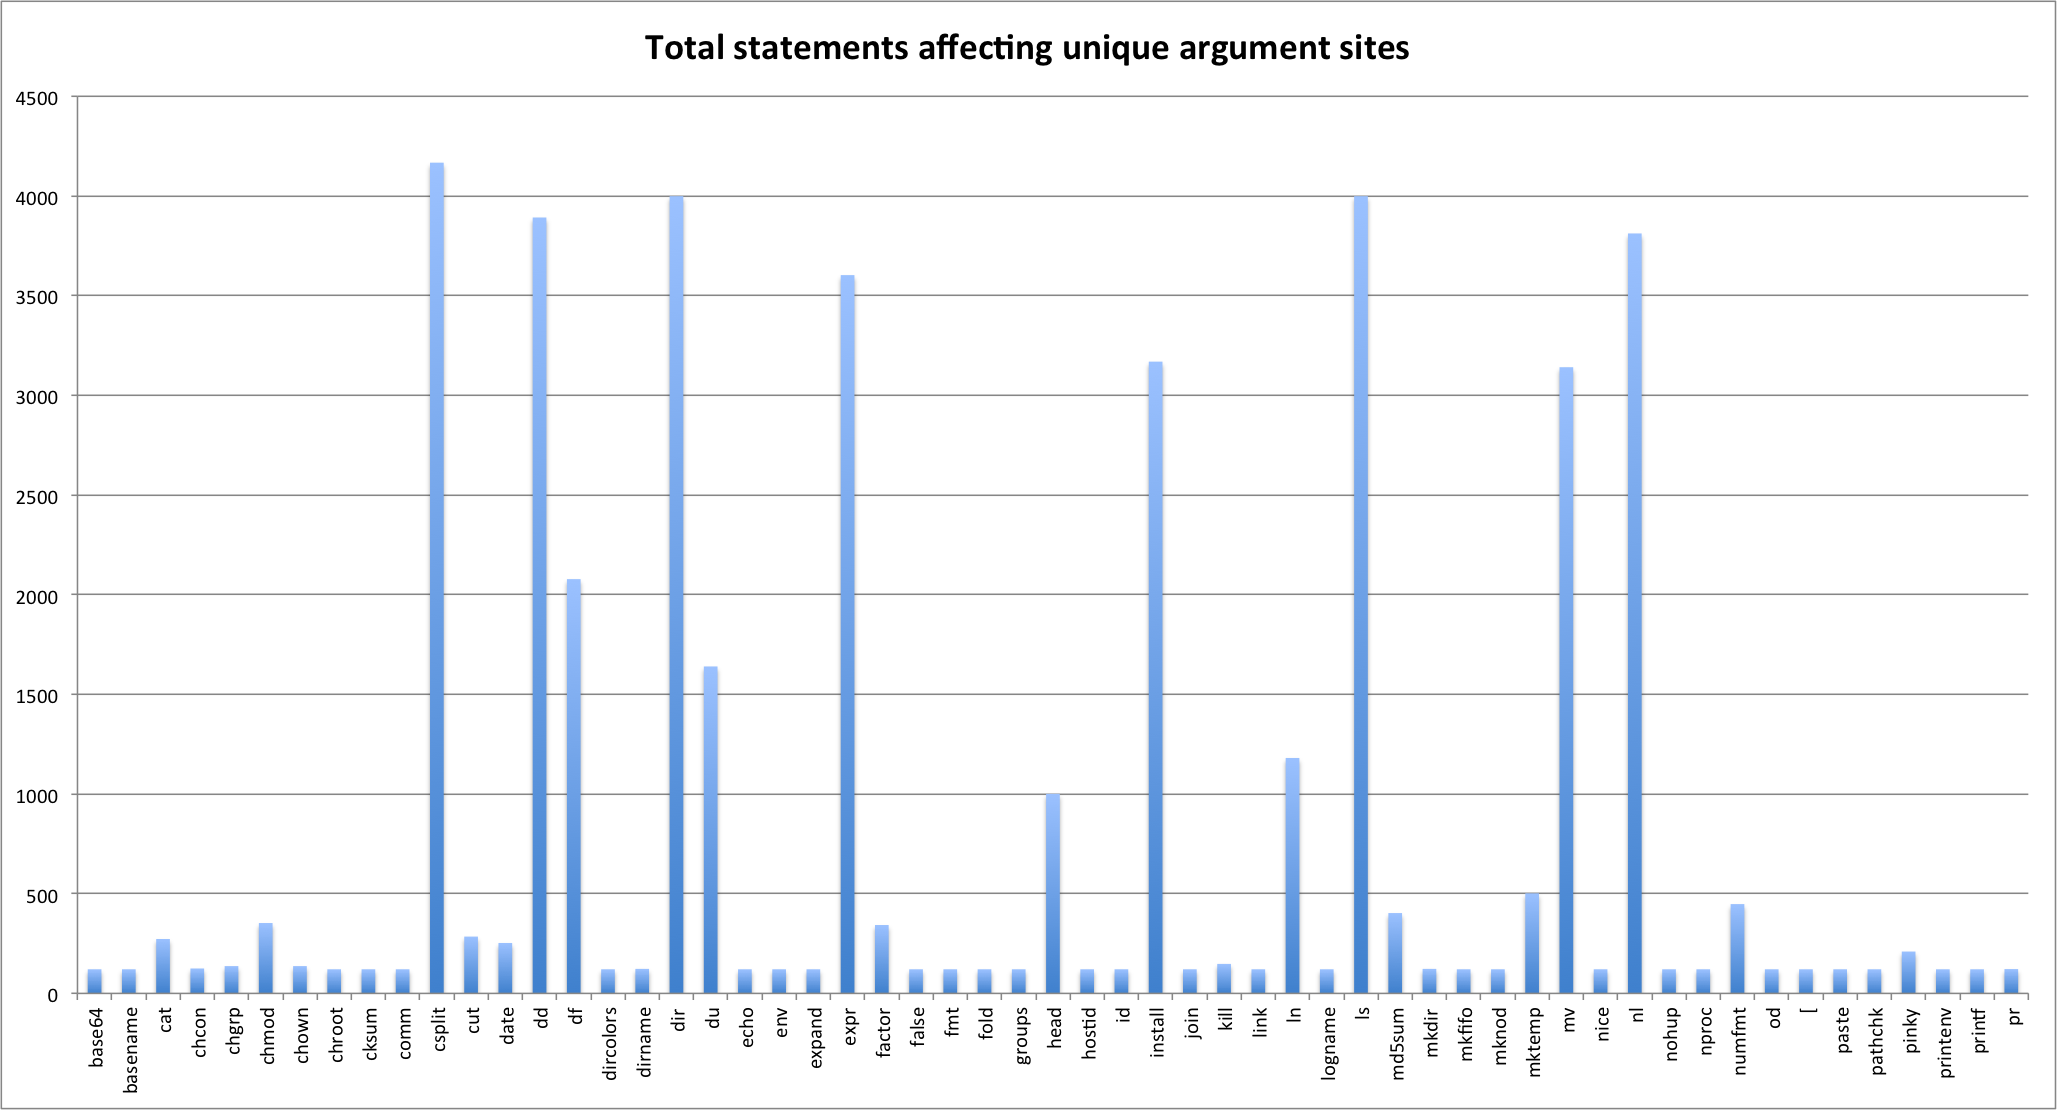
\includegraphics[scale=0.45, trim=0mm 0mm 0mm 0mm, clip]{img/coreutilstotal.pdf}
% \caption{Total statements }
\label{fig:coretotal}
\end{figure}

\paragraph{}
The figures illustrate some interesting properties with respect to argument
sites and data dependencies. Consider that each potentially dangerous function
takes 2 or 3 parameters--of these, our data dependency plugin determined the
maximum number of statements a single argument site statement is dependent on.
We observe from Figure~\ref{fig:corestats} that this could number in the hundreds,
whereas the total number could range in the thousands (Figure ~\ref{fig:coretotal}).
The implication here is that any additional reasoning and refinement to static
analysis methods across cases composed of sizeable dependencies need to be
carefully considered. For instance, if we add forms of pointer analysis,
we may speculate about the scale of complexity of memory operations for
argument sites.

\paragraph{}
We did not observe any violations with respect to the security outcomes
in~\S\ref{stackoutcomes}. This is perhaps unsurprising, given the ubiquitous
use of the \texttt{Coreutils} suite. At the same time, it is difficult to
choose a test suite which purposefully exhibits the stack properties that we
check; see \S\ref{lessonslearned} for further discussion.

\subsection{Malloc}
% dominic todo


% ======================================================================
\section{Experimental Evaluation}

\paragraph{}
In general, we were pleased that our plugins ran successfully on our own
example binaries as well as \texttt{Coreutils}. A key aspect of evaluating
the success of our project is that we were able to start with a basic API in
BAP, and after implementing a non-trivial amount of `infrastructure' code,
arrive at three individual plugins which are able to produce security outcomes.

\paragraph{}
Our evaluation of these plugins are largely qualitative rather than
quantitative at this stage. However, they serve as very useful data points
toward developing more sophisticated analyses.

\subsection{Malloc Check Plugin} 
% tiffany TODO


\subsection{Stack Check Plugin}

\paragraph{}
As mentioned, our stack check plugin did not trigger any violations when run
over the \texttt{Coreutils} test suite. This result was largely anticipated:
the \texttt{Coreutils} library was chosen so that we could verify that our
plugins run and to rule out the possibility that binaries in \texttt{Coreutils}
exhibited rudimentary flaws. 

\paragraph{}
In critique of this plugin, there are a number of stack-based errors that could
occur despite our checks. For example, consider a stack frame containing
multiple local buffers at runtime. It is feasible that a buggy \texttt{strcpy}
call could copy bytes beyond the boundary of a single buffer into an adjacent
buffer, while remaining within the stack bounds. Our plugin would not detect
this case. Consider a further case where memory accesses to the stack 
are dependent on general purpose registers---here we cannot conclude
whether the access is within range of the stack frame.

\paragraph{}
A positive side-effect of the plugin is the potential of reusability, and by
extension, refinement toward more sophisticated analyses. Recall that this
plugin collects and makes use of statements that an argument site depends on.
Thus, we have the ability to store the output of our analysis without having to
rerun the plugin. For example, we may be able to couple this data with
pointer-analysis, and infer stack boundaries.

\subsection{Malloc Plugin}
% dominic TODO

\section{Surprises and Lessons Learned}
\label{lessonslearned}
%TODO tiffany, dominic

\subsection{Reasoning about buffer overflows}
\paragraph{}

An initial approach towards ensuring stack buffer overflow detection was to
attempt to reason about sizes of buffers which are passed to ``Potentially
Dangerous Functions''~\cite{seacord2008cert} such as \texttt{strcpy}. This
turned out to be an unfruitful approach for the scope of the project, since one
would have to invariably have to reason about memory accesses.

A concrete example that illustrates the difficulty of performing checks on
\texttt{strcpy} was found when we considered \texttt{libxkbfile.so.1.0.2}.
Initially we thought that this is a candidate we could perform our check on,
due to containing a \texttt{strcpy(buf,"none")} call. However, this was found
to compile to the \texttt{LDMIA.W} instructions mentioned before. This example
principally highlights the difficulty in choosing candidates for testing.

\subsection{General Things Learned}

In general, this project made clear the difficulty of tackling binary
problems.

We learned that it is more effective in our research to develop our approaches
with respect to security outcomes. By doing so, we incrementally identify the
requirements for producing desired security outcomes (e.g., reaching
definitions, use-def). It also seems to be a pattern that more sophisticated
analyses are built on top of simpler analyses (like those produced in this
project), rather than sophisticated analysis being stand-alone. This follows
because we require more fundamental information before reasoning about
further complexities.

\section{Conclusions and Future Work}


Just as valuable to find out what works as what doesn't... that really
is a meaningful contribution. Further applications: nevernote, fgets, coverity?

Influence of statements...

\section{Distribution of Total Credit}

\clearpage

\appendix
\section{Appendix}
\label{appa}
\paragraph{BIL Dissasembly of Listing \ref{strcpy}}

\begin{verbatim}
  SP := SP - 0x8:32
  mem := mem         with [base_436 + 0xFFFFFFF8:32, el]:u32 <- R11
  mem := mem         with [base_436 + 0xFFFFFFFC:32, el]:u32 <- LR
  base_436 := SP
  R11 := SP + 0x4:32
  t_439 := 0x4:32
  s_438 := SP
  SP := SP - 0x18:32
  t_442 := 0x18:32
  s_441 := SP
  mem := mem         with [R11 + 0xFFFFFFE8:32, el]:u32 <- R0
  mem := mem         with [R11 + 0xFFFFFFE4:32, el]:u32 <- R1
  R3 := R11 - 0x10:32
  t_447 := 0x10:32
  s_446 := R11
  R2 := 0x0:32
  mem := mem         with [R3 + 0x0:32, el]:u32 <- R2
  R3 := R3 + 0x4:32
  t_452 := 0x4:32
  s_451 := R3
  R2 := 0x0:32
  mem := mem         with [R3 + 0x0:32, el]:u32 <- R2
  R3 := R3 + 0x4:32
  t_457 := 0x4:32
  s_456 := R3
  R2 := 0x0:32
  mem := mem         with [R3 + 0x0:32, el]:u16 <- t_460
  t_460 := low:16[R2]
  R3 := R3 + 0x2:32
  t_463 := 0x2:32
  s_462 := R3
  R3 := mem[R11 + 0xFFFFFFE4:32, el]:u32
  R3 := R3 + 0x4:32
  t_467 := 0x4:32
  s_466 := R3
  R3 := mem[R3 + 0x0:32, el]:u32
  R2 := R11 - 0x10:32
  t_471 := 0x10:32
  s_470 := R11
  R0 := R2
  R1 := R3
  jmp 0x82E0:32
  LR := 0x849C:32
\end{verbatim}

\paragraph{BIL data dependency instructions for \texttt{argv[1]}}

\begin{verbatim}
  <(0x8444:32, 0)> base_436 := SP
  <(0x8444:32, 1)> mem := mem         with [base_436 + 0xFFFFFFFC:32, el]:u32 <- LR
  <(0x8444:32, 2)> mem := mem         with [base_436 + 0xFFFFFFF8:32, el]:u32 <- R11
  <(0x8444:32, 3)> SP := SP - 0x8:32
  <(0x8448:32, 2)> R11 := SP + 0x4:32
  <(0x8450:32, 0)> mem := mem         with [R11 + 0xFFFFFFE8:32, el]:u32 <- R0
  <(0x8454:32, 0)> mem := mem         with [R11 + 0xFFFFFFE4:32, el]:u32 <- R1
  <(0x8458:32, 2)> R3 := R11 - 0x10:32
  <(0x845C:32, 0)> R2 := 0x0:32
  <(0x8460:32, 0)> mem := mem         with [R3 + 0x0:32, el]:u32 <- R2
  <(0x8464:32, 2)> R3 := R3 + 0x4:32
  <(0x8468:32, 0)> R2 := 0x0:32
  <(0x846C:32, 0)> mem := mem         with [R3 + 0x0:32, el]:u32 <- R2
  <(0x8470:32, 2)> R3 := R3 + 0x4:32
  <(0x8474:32, 0)> R2 := 0x0:32
  <(0x8478:32, 0)> t_460 := low:16[R2]
  <(0x8478:32, 1)> mem := mem         with [R3 + 0x0:32, el]:u16 <- t_460
  <(0x8480:32, 0)> R3 := mem[R11 + 0xFFFFFFE4:32, el]:u32
  <(0x8484:32, 2)> R3 := R3 + 0x4:32
  <(0x8488:32, 0)> R3 := mem[R3 + 0x0:32, el]:u32
\end{verbatim}

\paragraph{Graphical output of BIL data dependencies, with highlighted arguments}

\begin{figure}[ht!]
\centering

\includegraphics[scale=0.15, trim=0mm 0mm 780mm 0mm, clip]{img/ddep.pdf}
% \caption{Some caption}
% \label{fig:diagram_description}
\end{figure}

\nocite{*}
{\bibliographystyle{acm}
\bibliography{b1}}

\end{document}
